\chapter{Revisão Bibliográfica}

% Para ilustrar a completa ades\~ao ao estilo de cita{\c c}\~oes e listagem de
% refer\^encias bibliogr\'aficas, a Tabela~\ref{tab:citation} apresenta cita{\c
% c}\~oes de alguns dos trabalhos contidos na norma fornecida pela CPGP da
% COPPE, utilizando o estilo num\'erico.
% 
% \begin{table}[h]
% \caption{Exemplos de cita{\c c}\~oes utilizando o comando padr\~ao
%   \texttt{\textbackslash cite} do \LaTeX\ e
%   o comando \texttt{\textbackslash citet},
%   fornecido pelo pacote \texttt{natbib}.}
% \label{tab:citation}
% \centering
% {\footnotesize
% \begin{tabular}{|c|c|c|}
%   \hline
%   Tipo da Publica{\c c}\~ao & \verb|\cite| & \verb|\citet|\\
%   \hline
%   Livro & \cite{book-example} & \citet{book-example}\\
%   Artigo & \cite{article-example} & \citet{article-example}\\
%   Relat\'orio & \cite{techreport-example} & \citet{techreport-example}\\
%   Relat\'orio & \cite{techreport-exampleIn} & \citet{techreport-exampleIn}\\
%   Anais de Congresso & \cite{inproceedings-example} &
%     \citet{inproceedings-example}\\
%   S\'eries & \cite{incollection-example} & \citet{incollection-example}\\
%   Em Livro & \cite{inbook-example} & \citet{inbook-example}\\
%   Disserta{\c c}\~ao de mestrado & \cite{mastersthesis-example} &
%     \citet{mastersthesis-example}\\
%   Tese de doutorado & \cite{phdthesis-example} & \citet{phdthesis-example}\\
%   \hline
% \end{tabular}}
% \end{table}

\lipsum[1-1]

% -.~.-.~.-.~.-.~.-.~.-.~.-.~.-.~.-.~.-.~.-.~.-
\section{Dinâmica de Sistemas Multicorpos}

\subsection{Cinemática}\label{sec::cinematica}

\subsection{Cinemática Inversa e planejamento de
trajetória}\label{sec::ikin_traj}


% exact cellular de composition
% Bountrophedon Path
% Coverage path planning

Os parâmetros como posição, velocidade e orientação ao longo de um dado caminho
são impostos ao robô através do planejamento da trajetória.

% O planejamento é feito aliando-se o caminho desejado aos requisitos necessários
% ligados a uma deter

A importância de incluir corretamente os parâmetros da trajetória se
deve ao fato de que são estes parâmetros que serão verificados ao se comparar
os resultados do robô no modelo de base rígida aos resultados do modelo do robô
sobre uma base flexível. 

Se a tarefa é, por exemplo, o processo de revestimento por HVOF de uma
superfície , o robô deve seguir uma trajetória ao longo daquela superfície, de
forma a cobrí-la totalmente com o material aspersado. Como visto na
seção~\ref{sec::ikin_traj} uma maneira simples de cobrir uma superfície é pelo
movimento de ``zigue-zague'', ilustrado
na Figura~\ref{fig::zigzag}.\todo{Rever / reescrever esse parágrafo}

\missingfigure{Figura esquemática da trajetória}.

O sistema de revestimento por HVOF que motiva este trabalho, realiza a tarefa
sobre uma superfície suavemente curva, que representa o perfil hidráulico, da pá
da turbina. Como um dos requisitos do processo é manter a distância fixa entre a
pistola de revestimento e a pá, a trajetória não está restrita a apenas um
plano.

\begin{figure}[h]
	\centering 
 	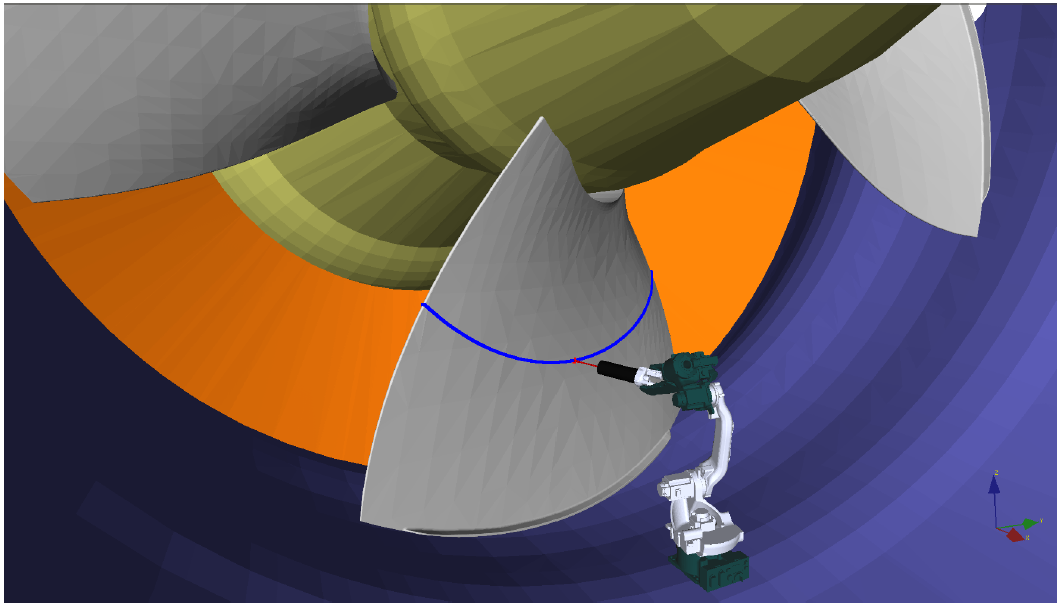
\includegraphics[width=0.75\textwidth]{figs/coat_blade}
 	\caption[Revestimento da face curva de uma pá]{Revestimento da face curva de
 	uma pá. \\Fonte: \citet{8206216}}
 	\label{fig::trajec_600x30}
\end{figure}

\subsection{Dinâmica}

\subsection{Equações de Movimento}

\subsection{Sophia-Maple e Método de Kane}\label{sec::sophia-kane}

\subsubsection{Notação de Lesser e Lennartsson}


% -.~.-.~.-.~.-.~.-.~.-.~.-.~.-.~.-.~.-.~.-.~.-
\section{Análise dinâmica de estruturas}

\subsection{Matriz de rigidez} \label{sec::rigidez}

\subsection{Amortecimento proporcional} \label{sec::amortecimento}

\subsection{Frequência Natural, Modo de Vibração e Amortecimento}
\label{sec::param_mod}

\subsection{Ensaio experimental de vibrações}


% -.~.-.~.-.~.-.~.-.~.-.~.-.~.-.~.-.~.-.~.-.~.-
\section{Manipuladores robóticos industriais}\label{sec::manind}

\subsection{Manipuladores flexíveis}

\subsection{Manipuladores sobre bases flexíveis}

\subsection{Tarefas de precisão utilizando manipuladores robóticos}

\subsection{Sistema de revestimento por asperção térmica} \label{sec::hvof}

\subsection{Tarefas robóticas \textit{in-situ}} \label{sec::insitu}



\begin{figure}[h]
	\centering 
 	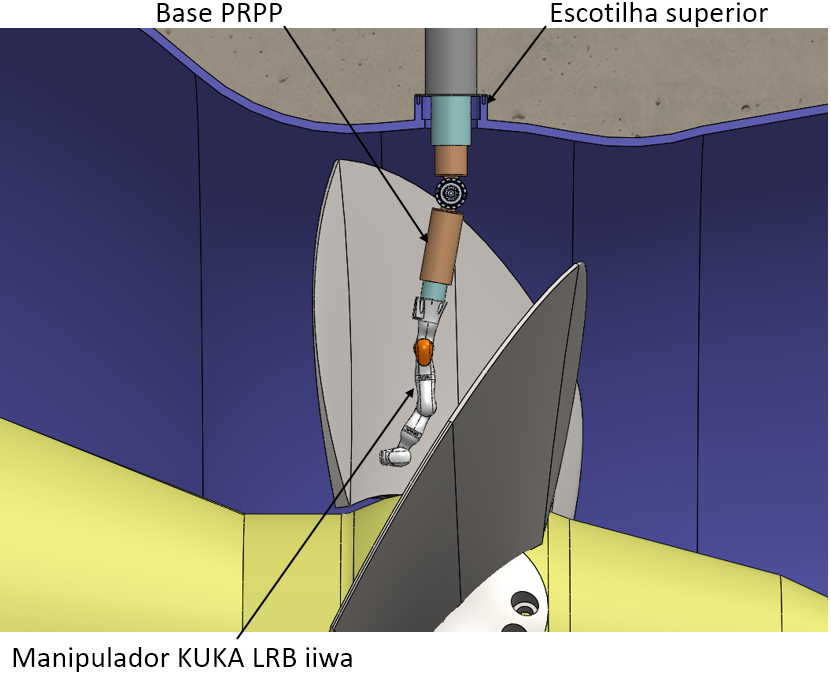
\includegraphics[width=0.85\textwidth]{figs/base_telesc_turbina}
 	\caption{Base telescópica PRPP para manutenção de revestimento
 	\textit{in-situ}}
 	\label{fig::base_telesc_turbina}
\end{figure}

\begin{figure}[h]
	\centering 
 	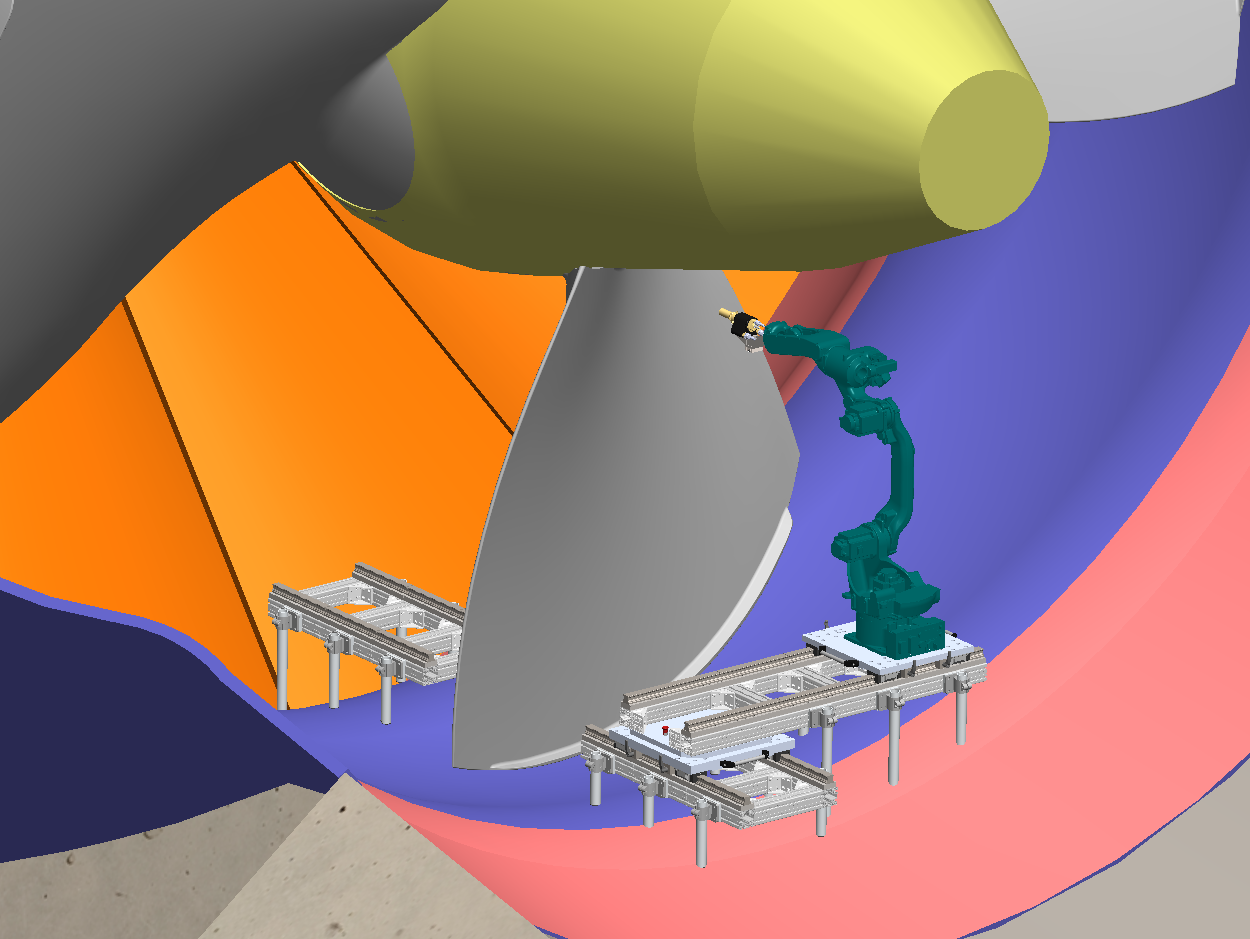
\includegraphics[width=0.85\textwidth]{figs/prp_turbina}
 	\caption{Base modular PRP para manutenção de revestimento \textit{in-situ}}
 	\label{fig::prp_turbina}
\end{figure}




















